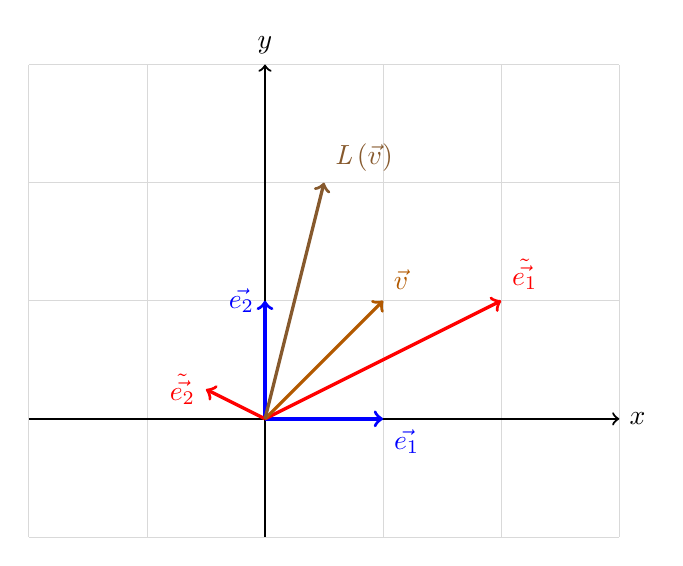
\begin{tikzpicture}[scale=1.5]
  \draw[step=1cm,gray!30,very thin] (-2,-1) grid (3,3);
  \draw[->,thick] (-2,0) -- (3,0) node[right] {$x$};
  \draw[->,thick] (0,-1) -- (0,3) node[above] {$y$};

  % Old basis (blue)
  \draw[->,very thick,blue] (0,0) -- (1,0) node[below right] {$\vec{e_1}$};
  \draw[->,very thick,blue] (0,0) -- (0,1) node[left] {$\vec{e_2}$};

  % New basis (red)
  \draw[->,very thick,red] (0,0) -- (2,1) node[above right] {$\tilde{\vec{e_1}}$};
  \draw[->,very thick,red] (0,0) -- (-0.5,0.25) node[left] {$\tilde{\vec{e_2}}$};

  % Vector v (orange)
  \draw[->,very thick,orange!70!black] (0,0) -- (1,1) node[above right] {$\vec{v}$};

  % Linear map (brown)
  \draw[->,very thick,brown!70!black] (0,0) -- (0.5,2) node[above right] {$\textit{L}\left(\vec{v}\right)$};
\end{tikzpicture}
